% I used overleaf

\documentclass[11pt]{amsbook}
\usepackage[turkish]{babel}
\usepackage{../Ceyhun}
\usepackage{../amsTurkish}
\usepackage{lipsum}

\begin{document}
% ++++++++++++++++++++++++++++++++++++++
\hPage{025}
% ++++++++++++++++++++++++++++++++++++++

$S_5: (1,1,0,0)$

$\qquad \ \underline{\uparrow \ \uparrow}$

$\qquad k_1 = 1$

$S_6: (0,0,0)$

ile sonuçlanacaktır. $S_6$ nın düğümsel olduğu hemen görülebilir. Öyleyse, $S_6$ dan başlayarak aranan çizge Şekil 1.3.3 de açıklandığı gibi elde edilebilir. 

Bu örnekten de kolayca anlaşılacağı gibi, düğümsel bir dizinin gerçekleştirimi \textit{birik} değildir.

Örneğin, Şekil 1.2.1 ve Şekil 1.3.3 deki çizgelerin kerte dizilerinin özdeş olmasına karşın, 

	\begin{center}
    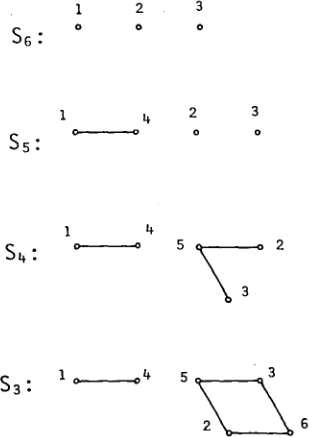
\includegraphics[width=0.35\textwidth]{images/ceyhun-025-fig01}
	\end{center}

\end{document}